\documentclass[UTF8]{book}
\usepackage{graphicx}
\usepackage{caption}
\usepackage{subcaption}
\usepackage{float}
\usepackage{amsmath}
\usepackage{amsfonts}
\usepackage{seqsplit}
\usepackage{tikz}
\usepackage{pgfplots}
\usepackage{listings}
\usepackage{CJK}

\newtheorem{theorem}{Proposition}
\newtheorem{definition}{Definition}
\newcommand\longnumber[2]{%
    \begin{minipage}{#1}
    \seqsplit{#2}
    \end{minipage}
    }
\newcommand*\thickdash{\includegraphics{thick-dash2}}
\newcommand*\thickdot{\includegraphics{thick-dot2}}

\graphicspath{ {images/} }
\begin{document}
\begin{CJK}{UTF8}{gbsn}

\title{The Network}
\author{Dan Auerbach}
\date{2015}
\maketitle

\part{The Telephone}

In 1876, to celebrate the centennial of the Declaration of Independence, the United states hosted its first World's Fair in Philadelphia. The event lasted several months, thirty-seven countries participated, and nearly 10 million visitors attended.

The biggest draws were mechanical inventions: displays of steam engines, the world's Remington Typographic Machine (the first typewriter), and precision watches, to name a few. Yet the age of electricity was just around the corner, and electrical contraptions were also on display. In a modest area across the Machinery Hall sat a young Alexander Graham Bell, demonstrating the transfer of human voice through wires.

People viewed early telephone prototypes like the one on display by Bell as a kind of toy, not a serious contender to the business-oriented telegraph empire of Western Union. That perception was due in part to the fact that prototypes at the time were limited in their range, typically connecting just two adjacent rooms, and it was not obvious at first that the technology could scale to rival the telegraph network. Yet once it became clear that longer-distance telephony was possible, it did not take long for commercial telephony to develop, seeded by Bell and his collaborators. Once off the ground, there was a rapid shift in power away from the well-established Western Union and instead towards the upstart corporation that would become AT\&T, a telecommunications giant that would come to define the industry in the United States for a century.

In this part of the book, we will examine how the telephone works: what is sound? how is an analog signal transmitted over a wire? To understand telephony, we will go step by step through the process of building a telephone from scratch, and then outline the key insights required to build a telephone network. In addition to learning about the technology, we will also examine some historical and social issues related to how the regulatory landscape began to evolve in the United States as the telecommunications industry matured.

Given that our ultimate goal is understanding the Internet and not the telephone network, we will NOT attempt to follow each step of the complex historical evolution of the telephone, nor describe every aspect of a real-world telephone system, which is of course extremely complicated. For readers interested in developing deeper knowledge of telephony, I recommend [INSERT BOOK REC].

\chapter{Signals}

In the previous chapter, we studied symbols quite extensively, emphasizing the transmission of symbols from one location to another as a \emph{digital} telecommunication system. In contrast to representing information as a series of discrete symbols, information can also be presented in an \emph{analog} fashion via \emph{signals}, in which a variable might take on an infinite number of values over time. Recall that such a variable is called \emph{continous}. A few examples of continuous variables are time, pitch, temperature, human height.

Early telephone systems represented human society's first foray into an analog telecommunication technology, allowing sound to be transmitted from one location to another, and so we will use this a natural jumping off point to understand analog signals.

\section{Sound}

When a tree falls and hits the ground, some of the energy upon impact is transferred to nearby air particles, pushing them outwards in a wave.

\begin{figure}[H]
\centering
\includegraphics[width=0.8\linewidth]{treefalling_edited}
\end{figure}

The wave is a \emph{longitudinal} wave, meaning it does not have the peaks and troughs of an ocean wave perpendicular to the direction of travel, but instead expands and contracts along a single dimension as it travels.

\begin{figure}[H]
\centering
\includegraphics[width=0.8\linewidth]{longvstransvwave}
\end{figure}

As a first approximation towards understanding sound, imagine a large explosion at the moment the tree strikes the ground, except that instead of an outwardly expanding sphere of fire, there is an outwardly expanding sphere where air particles are more tightly bunched together for perhaps a second or less. This momentary compression of air particles constitutes a change in \emph{air pressure} in that location.

As objects on Earth interact with each other, waves of pressure expand outward in the surrounding medium (in the example above, this medium is the air). These pressure changes often signal events that are important to an organism, like when something might eat it or when it might be able to eat something. Given the importance of this information for survival, many species including humans evolved auditory systems to make sense of the constantly and subtly changing air pressure all around us; we call our experience of this phenomena \emph{hearing}. And in parallel to the development of our sense of hearing, we evolved increasingly sophisticated ways to create sound ourselves, culminating in vocal chords and speaking.

The simplified description above of a tree falling might lead one who is unfamiliar with hearing to believe that there is only a single, uniform experience of a sound, but of course that's not the case. Sound has many different qualities, like pitch, intensity, duration, and timbre. It is quite easy to tell the singing of a friend from the sound of a tree hitting the ground. This differentiation is possible because sound waves can be rather sophisticated, the miniscule air particles compressing and un-compressing in non-uniform ways over very small distance and time scales. In particular, as we will see, a single moment of the bunching of air particles is NOT detectable by our ears. Instead,we pick up on very rapid compression and un-compression that forms a wave pattern and occurs as the result of a vibration. [IAMHERE THIS NEEDS WORK]

To illustrate these differences, here is a representation of the sound of a tree falling:

\begin{figure}[H]
\centering
\includegraphics[width=0.8\linewidth]{tree_falling_soundwave}
\end{figure}

And here is a representation of human speech:

\begin{figure}[H]
\centering
\includegraphics[width=0.8\linewidth]{shakespeare_speech}
\end{figure}

The above figures are called \emph{time domain representations}: the x axis is time, and the y axis represents the instantaneous change in air pressure. Large values on the y axis mean that particles are tightly compressed at that instant. Of course these representations have to be taken from a single source point: two people standing in different places may have different auditory experiences of the same tree-falling event.

\section{Functions}

The two figures above representing various sounds are examples of \emph{functions}, a central concept in mathematics.

A function is a mapping from one set of objects to another:

\begin{figure}[H]
\centering
\includegraphics[width=0.8\linewidth]{function_basic}
\end{figure}

We say that a function has a \emph{domain}, which is the set of objects on the left in the figure above, and a \emph{co-domain} which is the set of objects on the right. There is one important rule that must be followed for something to count as a function:

\begin{itemize}
\item For each object in the domain, a function MUST map that to EXACTLY ONE object in the co-domain
\end{itemize}

In other words, since functions must be defined on the entire domain, this isn't allowed:

\begin{figure}[H]
\centering
\includegraphics[width=0.8\linewidth]{function_undefined}
\end{figure}

And neither is this:

\begin{figure}[H]
\centering
\includegraphics[width=0.8\linewidth]{function_multifunction}
\end{figure}

Note that the converse of the second rule above does not hold; it is perfectly acceptable for several values in the domain to be mapped to a single value in the co-domain, as is the case in the first diagram above.

So far, the domain has been 4 blobs, and the co-domain has been 3 blobs, but this is just one example. There are no restrictions on the domain or co-domain. You can have a function where the domain is pet owners on Earth, and the co-domain is the set of pets:

\begin{figure}[H]
\centering
\includegraphics[width=0.8\linewidth]{function_pets}
\end{figure}

We might call this function ``FavoritePet'', and write $FavoritePet(John) = Fluffy$ to mean that the function ``FavoritePet'' maps the element ``John'' in the domain of pet owners to the element ``Fluffy'' in the domain of pets, a formal way of writing that Fluffy is John's favorite pet. (\emph{Exercise}: would ``Owns'' with the same domain and co-domain constitute a function? why or why not?)

To indicate that a function $f$ has domain $A$ and co-domain $B$, we use the notation $f: A \rightarrow B$. In this case the function itself is $f$ and the value of the function at $x$ is denoted by $f(x)$.

The domain and co-domain of a function can be finite (like Pet Owners) or infinite (like natural numbers: $\mathbb{N} = {0, 1, 2, 3, etc.}$). The domain and co-domain could be the same, but they do not have to be.

Sometimes functions can be described easily, like ``FavoritePet'' or the function $f: \mathbb{N} \rightarrow \mathbb{N}$ that takes a natural number and doubles it. We could call this function ``Doubles'', but mathematicians prefer a more compact and precise description: $f(x) = 2x$. Here $x$ is a variable and so the description of $f$ above works for the entire domain, although the expression does not specify the domain explicitly.

Other times functions cannot be described easily at all but instead are simply a random-looking mapping from the domain to the co-domain. In this case, the only way to give a full description of the function is to give it's value for every single input object, a task that is sometimes provably impossible when there are an infinite number of input objects. But even in these cases, the functions themselves are valid in a mathematical sense, even if they defy easy description or understanding.

Domains or co-domains might be multi-dimensional spaces. For example, a function $f: \mathbb{N}^{3} \rightarrow \mathbb{N}$ would map triplets like $(4,5,1)$ to natural numbers like $17774$. Domains and co-domains can also be discrete, like the natural numbers. Or they can be continuous, in that they range over a continuous variable such as time. [FOOTNOTE: the mathematical definition of a continuous variable is subtle, but an approximation is the notion of \emph{density}: for a variable A, and any values $x$, $y$ that can be taken on by $A$ such that $x < y$, there is a value $z$ that the variable $A$ can take on and $x < z < y$. Exercise: show that this property does NOT hold for the natural numbers $\mathbb{N}$.]

How does this discussion of functions relate to the plots of sound waves above? It turns out that that familiar plot along an x and y axis is a representation of a function, where the x axis is the domain and the y axis is the co-domain.

After all, a function is an abstract object, and as such it has many representations. For example, the function $f(x)=2x$ can be described by plotting it on a two dimensional axis, where the x-axis is the input of the function and the y-axis is the output:

\begin{tikzpicture}
\begin{axis}[
    axis lines = left,
    xlabel = $x$,
    ylabel = {$f(x)$},
]
\addplot [
    domain=-10:10,
    samples=100,
    color=red,
]
{2*x};
\addlegendentry{$f(x) = 2x$}
\end{axis}
\end{tikzpicture}

It could also be represented with the primary visualization that we used to introduce the notion of a function:

\begin{figure}[H]
\centering
\includegraphics[width=0.8\linewidth]{function_2x}
\end{figure}

We will return to functions quite often, so it is important to develop a sharp understanding of this mathematical object. \newline

\emph{Exercise}: write out a mathematical description for a function $f$ that takes two numbers, and raises the first to the power of the second, then subtracts the second. What is the value of $f(3,4)$? As a bonus, use graphing software to create a graphical representation of this function as a 2-dimensional surface sitting in a three-dimensional space.

\section{Speech on a wire: an analog approach}

Above, we saw examples of functions that represented sound. Here again is our time domain representation of speech, also called a speech \emph{waveform}:

\begin{figure}[H]
\centering
\includegraphics[width=0.8\linewidth]{shakespeare_speech}
\end{figure}

As we have seen, this is just a function in which the domain is time and the co-domain is air pressure. The information in the figure above is enough to create a sound that we would recognize as speech. In order for telephony to be possible, we need a way to continuously transmit the information of the sound waveform from one location to another, farther and faster than we could via sound waves (in other words, by just shouting).

An electrical wire does not contain air particles that can be compressed and uncompressed, but it does have other properties that can be varied continuously over time. In particular, the current flowing through a wire can increase and decrease.

Let's go back to the telegraph for a moment. In the case of the telegraph, the current was on or off, resulting in a function of electrical signal over time that might look something like this:

\begin{tikzpicture}
\pgfplotstableread{
0 0
1 0
2 0
3 1
4 0
5 1
6 1
7 1
8 0
9 1
10 0
11 0
12 0
13 0
14 0
15 0
16 0
17 0
18 0
19 0
}\datatable
\begin{axis}[
    axis lines = left,
    xlabel = time,
    ylabel = electrical current,
    ytick = {0,1},
]
\addplot+[thick, const plot, mark = none] table [x index=0, y index=1]{\datatable};
\addlegendentry{$\thickdot \thickdash \thickdot$}
\end{axis}
\end{tikzpicture}

(In reality, the telegraph signal was distorted by the time it was received and so did not look quite so clean, but conceptually this was the signal being sent.)

The telephone, in contrast, has to solve the more difficult problem of reproducing the information of the speech waveform above via changes over time to electrical current.

[INSERT IMAGE OF WAVEFORM ABOVE BUT AS CURRENT]

[CHART OF CONCEPTUAL OUTLINE OF TELEPHONE]

\section{Basics of signals}

We will see how the telephone accomplishes this shortly, but first let us turn our attention to the idea of a \emph{signal}.

We have already covered basic symbolic systems, and the fact that any symbolic representation of information is interchangeable [ADD NAME FOR THIS THEOREM?]. But what happens when the information we care about is an analog function over time like the human voice that cannot be easily represented as a set of symbols?

In this case, we are instead dealing with a \emph{signal}. While there is no standard definition of a signal, for our purposes let us consider it to be a function where the domain is time, and the co-domain is a continuous variable that bears information. This definition allows us to abstract away the function that contains information from the particular medium upon which it resides. So, for example, we can consider the speech waveform above and its translation into electrical current to both be different representations of the same signal.

So far we have looked at a speech signal, and the signal produced by a tree hitting the ground. What about the sound of a C note that does not vary in pitch or intensity? You might expect the signal associated with such a uniform sound to look like the function that graphs pitch over time:

[STRAIGHT LINE]

However, a single C note in fact is a signal that looks like this:

[SINE WAVE]

This signal is \emph{periodic}. This very simple periodic function is sometimes called a \emph{sine wave}, corresponding to the trigonometric sinusoidal function. [ADD FOOTNOTE EXPLANATION OF SINE?]. Most sound signals, including signals corresponding to voices, are actually a composition of many such periodic signals.

Periodic signals have a \emph{frequency}, indicating the number of cycles per second, and an \emph{amplitude} indicating the magnitude of the peaks and troughs of the signal. In the case of a sound signal, it turns out that changes in frequency correspond to changes in pitch. To give a concrete example, the note A above middle C in a piano creates the following signal:

\[ f(x) = sin(880\pi x) \]

Here the domain is time in seconds, and we can graph the function:

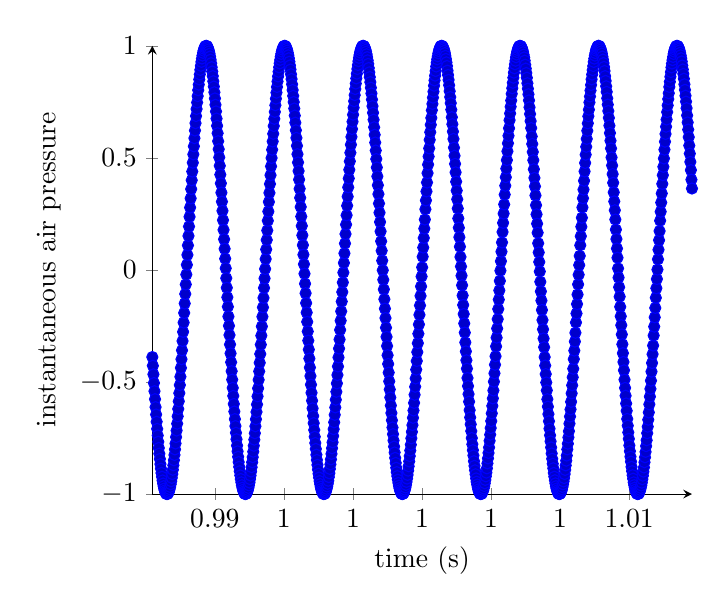
\begin{tikzpicture}
\begin{axis}[
    axis lines = left,
    xlabel = time (s),
    ylabel = {instantaneous air pressure},
    samples = 1000,
    domain=127/128:129/128,
    legend pos=outer north east,
]
\addplot
{sin(deg(880*pi*x))};
\end{axis}
\end{tikzpicture}

The frequency of the function $sin(x)$ is $2\pi$ since that comprises a full rotation around the unit circle. Hence, the function $f(x)$ above corresponding to our A note has a frequency of 1/440, meaning that there are 440 oscillations per second. The unit ``per second'' has a name, which is \emph{hertz}, abbreviated \emph{Hz}, and so we say that the frequency of an A note is 440Hz. If you are a musician with a basic knowledge of music theory, you probably know this fact.

The fact that this frequency is fairly high helps to explain why the experience of hearing an A note can appear monotone and uniform. Our auditory system is not designed to discern the individual peaks and troughs whizzing by, but rather to pick up on the frequency of oscillations.

As such, tones are distinguished by their frequency and higher-frequency sound waves have a higher pitch, a fact also familiar to those familiar with music.

[IAMHERE, ADD functions for different pitches]

Given the sensitivity of the human auditory system to small oscillating vibrations, our vocal chords evolved to make sound by creating vibrating sinusoidal sound waves, but we are not single-note rookies. We have mastery over creating these sinusoidal waves and can start, stop, and move up and down quickly between different frequency waves with ease, allowing the incredible feat of human speech.

It may not seem like the speech waveform displayed above is made up of sinusoidal components, but that is only because we have a sophisticated innate mastery over producing sounds, combining and adjusting different frequencies. Here is a zoomed in look at a section of the waveform over a very small time slice:

[SHOW SECTION OVER SMALL TIME SLICE]

As it happens, the mathematics behind combining these sinusoidal signals is quite important for telecommunication technology, and is basically as simple as addition.

[ADD MORE HERE ABOUT COMBINING SIN WAVES ETC]

\section{Information content and analog signals}

How much information does a sound signal contain? Of course it's not fair to compare a hundred years of sounds to a millisecond, so to start to get a handle on the information content of a sound, let's fix our metric to be information \emph{per second}.

But even now the answer is far from straight forward. A completely uniform sound intuitively has no information

[IAMHERE]

\chapter{How A Telephone Works}

The telephone transforms a sound signal into an electrical signal and back again. It was not the only analog device in the late 1800s that sought to manipulate sound in new ways.

The phonograph was invented in 1877 and was the original technology in a line that continued with record players, cassette tapes players, CD players, and MP3 players. [FOOTNOTE: it seems this line of technology may have been subsumed by more general purpose desktop and mobile computers in the last 5 years or so]. The phonograph was aimed at solving a dual problem to the telephone, in that it needed to capture a sound signal somehow. The difference is that once captured, instead of the moving the sound signal quickly over a long distance, the phonograph was instead tasked with creating a physical object from which the sound could be later retrieved, a record. Early phonographs used a circular disk as the record, and a sound signal was captured by deviations in a spiral groove. [MORE HERE?]

[DIAGRAM OF TELEPHONE VS PHONOGRAPH]

In this chapter, we will work towards building a telephone. It is worth mentioning that the telephone we build is not historical, nor does it do justice to the incredible complexity of the telephone system in even the early 20th century. Instead, deliberate choices have been made to stick to the simple core concepts, borrowing freely from different historical periods to offer the simplest version for readers who are new to telephony, in keeping with the goal of developing a solid conceptual understanding of the technology.

\section{Ohm's Law}

Before we can build a telephone, we need to understand a bit more about electricity. The most important principle for the purpose of building simple electrical components and devices is called Ohm's Law, an empirical law discovered in the early 19th century. To motivate Ohm's law, note that there are two critically important electrical quantities that we can measure whenever electricity is flowing through a system.

The first quantity is the electrical \emph{current}, commonly abbreviated $I$ in the field of electrical engineering. This is a measure of the ``flow'' of the electricity through the circuit, analogous to the amount of water that might flow through a pipe system per second. Electrical current can be measured using a device called a \emph{galvanometer}: a magnetic compass needle is deflected more or less depending on how much current is flowing through a wire. Just as we might choose a unit such as liters per second to describe the flow of water, a popular unit of measurement for electrical current is \emph{amperes (amps)}.

The second quantity of interest is called \emph{voltage}, abbreviated $V$. Borrowing again from the popular explanatory analogy to a water pipe, the voltage would be analogous to the pressure of the pipe. The voltage is measured in \emph{volts}, and can be measured independently of current, with the details of measurement depending on the type of circuit being used.

What is the relationship between current and voltage? That is the question that Georg Ohm set out to answer. Just as increasing the water pressure would increase the number of gallons per second flowing through the pipe system, so too an increase in voltage corresponds to a proportional increase in current. But until experiments are performed, the nature of this relationship is unclear. Ohm did the science: he formed a circuit with some copper wire, varied the voltage, and measured the current. He did this with different wires of different thicknesses (the \emph{gauge} of a wire is a standard measurement of diameter or, equivalently, cross sectional area). What he determined was that for any given wire, $I$ was linearly proportional to $V$. The constant changed from one length of wire to another, however.

Here is a fake example illustrating the sorts of calculations that Ohm performed almost 200 years ago:

[INSERT CHARTS]

How do we make sense of this data? Once we posit that each length of wire, or electrical component has a specific internal electrical \emph{resistance} then ALL of the data above can be condensed into a simple equation:

$I = V/R$

The final term $R$ stands for \emph{resistance}, and is the property of a particular electrical component.

\section{Electrical components}

Before we build a telephone, let's take stock of what electrical components we have at our disposal and formalize our electrical circuit diagrams a bit. We have already met the \emph{relay}, the \emph{switch} and the \emph{power source} (e.g. a battery). Here is how these components are typically represented in circuit diagrams:

[INSERT IMAGES]

\section{A one-way telephone}

A one-way telephone has a microphone at one end capable of translating an analog sound signal into an electrical one, and a receiver at the other end capable of translating the electrical signal back into an audible sound signal:

[DIAGRAM]

\subsection{Microphone}

A \emph{microphone} serves as the input mechanism, translating our sound signal into a signal of electrical currents. The main type of microphone for years was the carbon microphone and it worked like this:

[INSERT IMAGE]

Much like our eardrums, a thin metal diaphragm is used that vibrates in response to sound waves. When it is pushed inward, as in the diagram above, the carbon granules are squeezed closer together, decreasing the resistance of the granules, and thus increasing the current flowing through the wire. This means that the wire now can carry the same signal as the sound waves.

You might imagine that the carbon granules have to be specially placed for this scheme to work, but this is not the case. We do not need to know the exact path that electrons might take for the macroscopic principle to hold: as the instantaneous air pressure increases, the diaphragm is pushed inward, packing the granules more tightly and decreasing their electrical resistance, proportionally to the increase in air pressure.

\subsection{Receiver}

A \emph{receiver} is a diaphragm attached to an electromagnet. As the electrical current goes up, the electromagnet has a stronger magnetic pull, causing the diaphragm to vibrate more. As it vibrates, it generates changes in air pressure which are emanated from the receiver as sound.

\section{Telephones of the early 1900s}

In the above conceptual diagram, the electrical circuit is always closed, meaning that current is flowing continuously through the circuit without any means to stop it (aside from cutting the cord). In practice, a mechanism is needed to open the circuit when it is not in use, which helps to save battery. It is also desirable for phones to work in the familiar two-way fashion in which a person can talk and listen at the same time.


\chapter{The Telephone Network}

The first telephones connected a pair of adjacent rooms, making the problem of knowing who was at the other end of the line pretty straight forward.

But the dream of industrialist Theodore Vail, president of AT\&T from 1885 to 1889 and again from 1907 to 1919, was universal telephone service for all:

[QUOTE FROM VAIL]

He was an unabashed monopolist, and genuinely believed that a telecommunications monopoly was in the best interest of the country.

[QUOTE FROM VAIL]

This created a host of challenges: overcoming competition, getting the government to agree with the monopolistic approach to telephony, and establishing service in the most remote and rural parts of America. But alongside these business related challenges, a couple of technical issues loomed large when it came to building out a telephone network. First, how are people going to be identified? Second, how is person A going to be able to talk to person B?

\section{Telephone Numbers}

Naming was becoming a problem for the telegraph in the late 1800s. Until that point, if a telegram was addressed to John Smith in Boston, the message could properly be routed to the Boston office but then what? A lot of responsibility for getting this right fell on the sender of the message to appropriately specify a recipient (\emph{John Smith of Commonwealth Ave in Back Bay}) and on the local courier boys who worked for the telegraph office to have some familiarity with the neighborhood and where people or businesses were located.

As cities grew and telegram volume grew, this ad hoc system was becoming unsustainable.



\end{CJK}
\end{document}
